\setcounter{chaptercntr}{2}

\sectionbreak \section*{
  \gostTitleFont
  \redline
  \thechaptercntr . 
  АНАЛИЗ СУЩЕСТВУЮЩИХ РЕШЕНИЙ
}

\titlespace

{\gostFont

  \par \redline В этой главе будут проанализированы методы, которые были использованы при решении схожей задачи в организации Kaspersy.

  \par \redline	Перед организацией ставилась цель разработать систему, которая позволяла бы предотвращать отказы, аварии и незапланированные простои промышленного оборудования, выявляя признаки проблемы задолго до того, как проблема повлияет на работу предприятия. Другими словами, необходимо произвести прогнозирование данных технологического процесса промышленного оборудования для выявления признаков, по которым можно говорить о будущих аномалиях. Под аномалией для Kaspersky понимается значительное отклонение реальных данных технологического процесса от прогноза.

  \par \redline	Причинами, по которым Kaspersky занялся данной задачей, стали устаревшие системы мониторинга, не способные эффективно искать причины возникновения аварий, а также огромный объём телеметрии, с которыми не могли справиться даже опытные операторы.

  \par \redline	Для решения таких проблем была создана система Kaspersky MLAD. Это система для наблюдения за большим количеством пользователей телеметрии, а также для выявления отклонений, которые могут нанести повреждения производству.

  \par \redline Данная система способна предотвращать неполадки различного рода, представленные дефектом или сбоем оборудования, или ошибкой персонала, с целью дальнейшего предотвращения развития опасной ситуации. Также система способна определять отклонения в действиях сотрудников, позволяя раскрыть бойкот, диверсию, срыв производства и так далее. В добавок система Kaspersky MLAD призвана выявлять атаки злоумышленников. Место и роль данной системы на производстве можно увидеть на рисунке \thechaptercntr .\theimagecntr.

  \begin{figure}[H]
    \centering
    \def\svgwidth{\textwidth}
    \includesvg[width=806mm]{images/MLADBlackBox.svg}
    \caption*{\gostFont Рисунок \thechaptercntr .\theimagecntr \spc {--} Место системы Kaspersky MLAD на производстве}
    \label{fig:MLADBlackBox}
  \end{figure} \addtocounter{imagecntr}{1}

  \par \redline Для работы системы Kaspersky MLAD не требуется изменять как-либо технологической процесс промышленного оборудования. Эта система никак не воздействует на него. К тому же она не вмешивается в передачу данных или в средства управления промышленным оборудованием. Данная система оповещает оператора о возможном сбое, и оставляет задачу принятия решения на операторе. Данным свойством будет обладать и модели, описанные в данной работе. 

  \par \redline Если рассматривать Kaspersky MLAD с технической стороны, то это программное обеспечение, которое использует нейронные сети, способные анализировать существующий поток телеметрии. Поскольку параметры телеметрии связаны друг с другом и влияют друг на друга, то система Kaspersky MLAD должна это учитывать, и она с этим справляется. Она способна выявлять взаимосвязи между параметрами и использовать их для построения прогноза. Этот прогноз в дальнейшем обрабатывается различными нейросемантическими средствами, выявляя тем самым аномалии. 

  \par \redline Система Kaspersky MLAD использует различные архитектуры нейронных сетей, такие как: CNN, DenseNet, TCN и RNN. Первые три сети используются для различного рода обработки данных, их анализа и выявление аномалий. А сети RNN используются для прогнозирования данных технологического процесса промышленного оборудования. Данная работа последует примеру Kaspersky MLAD и также будет использовать RNN сети для прогнозирования. 

  \par \redline Таким образом, Kaspersky MLAD состоит из различных модулей нейронных сетей, взаимодействующих друг с другом. Рассматривая модель прогнозирования данной работы под призмой Kaspersky MLAD, можно понять, что задача данной работы состоит в том, чтобы создать один из этих модулей, выполняющий задачу прогнозирования. В дальнейшем планируется развитие данной работы и создание остальных модулей по примеру системы Kaspersky MLAD.

  \par \redline Но как именно система Kaspersky MLAD определяет аномалии. Для этого у системы имеется пять видов детекторов аномалий. Но интересует нас лишь, так называемый, предиктовый детектор, который строится на основе нейронных сетей. Суть его работы проста: сначала выполняется прогноз данных, затем этот прогноз сравнивается с фактическим наблюдаемым поведением и с помощью машинного обучения определяются аномалии. Данный модуль можно разделить на две модели: модель прогнозирования и модель обработки прогнозов. Тем самым, данная работа, если рассматривать её под призмой системы Kaspersky MLAD, ставит своей целью создание первого модуля предиктового детектора. Также нас интересует ещё один из видов детекторов аномалий, а именно потоковый процессор. Его задача состоит в том, чтобы приводить данные телеметрии к равноинтервальному временному виду, что подразумевает собой равным промежутки между точками относительно оси времени. Такой вид данных необходим для работы остальных видов детекторов аномалий, в том числе и для предиктового детектора. Аномалии в потоковом процессоре вычисляются в процессе приведения данных к равноинтервальному временному виду.

  \begin{sidewaysfigure}
    \centering
    \def\svgwidth{\textwidth}
    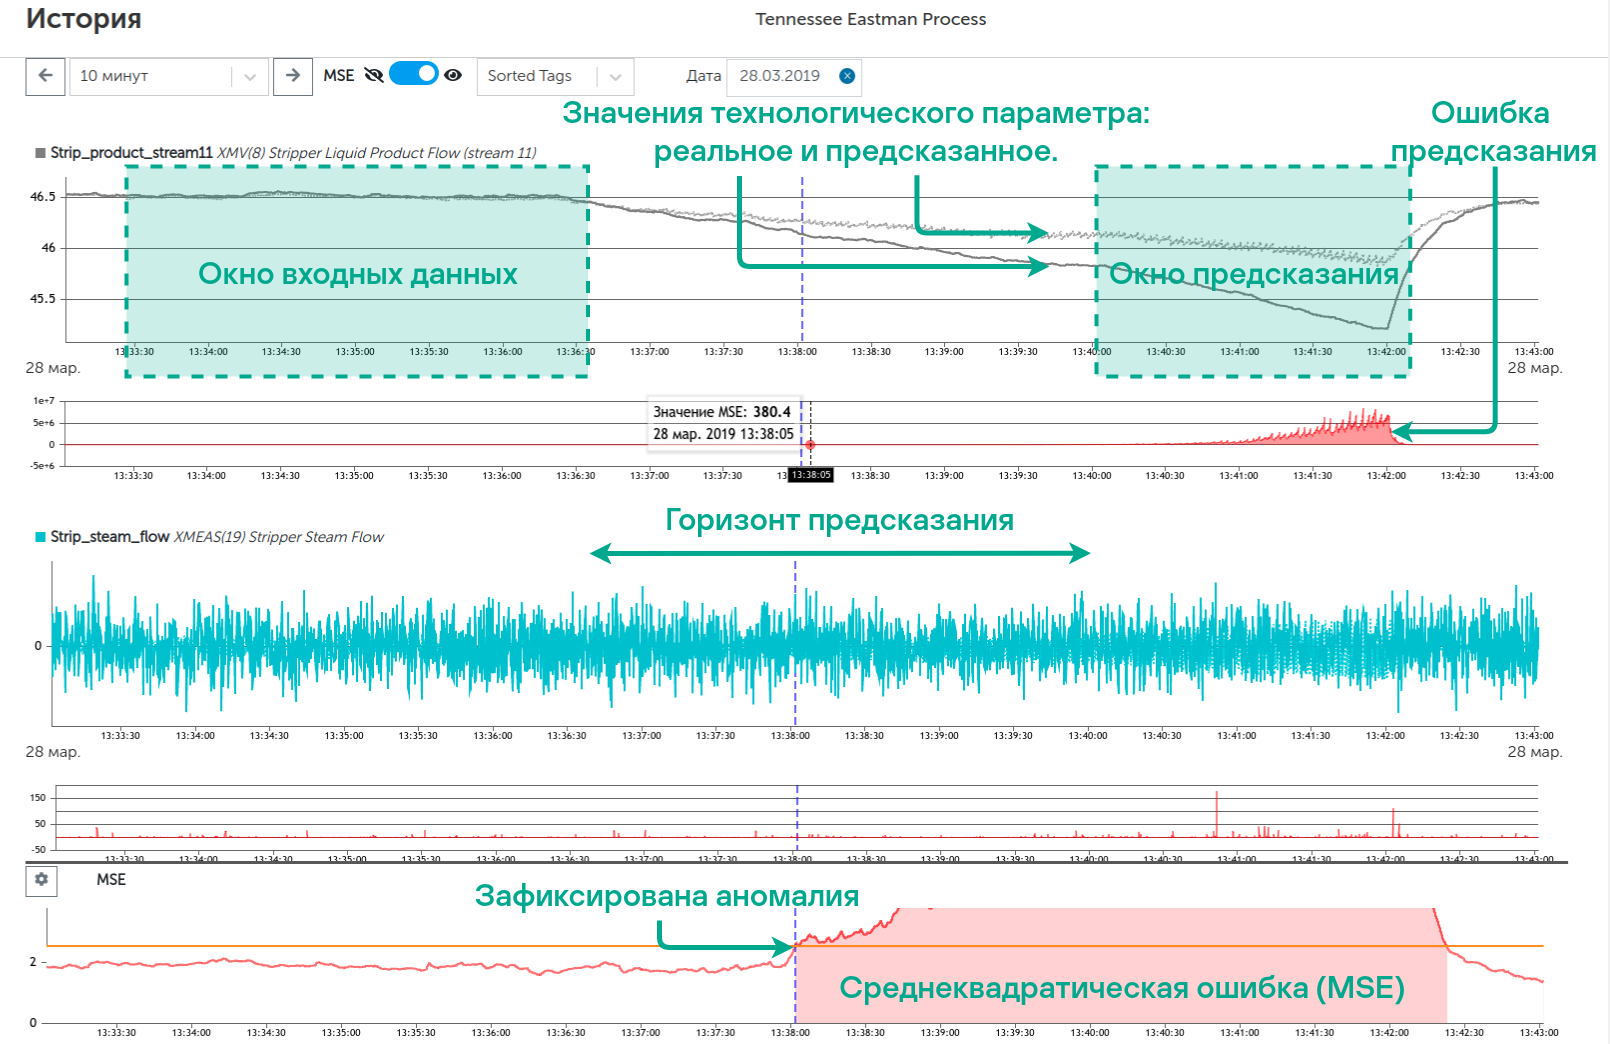
\includegraphics[scale=0.6]{images/MLADex.png}
    \caption*{\gostFont Рисунок \thechaptercntr .\theimagecntr \spc {--} Пример работы предиктового детектора системы Kaspersky MLAD}
    \label{fig:MLADBlackBox}
  \end{sidewaysfigure} 

  \par \redline Раз была определена схожесть данной работы с предиктовым детектором аномалий системы Kaspersky MLAD, тогда необходимо более подробно рассмотреть этот модуль и то, как он функционирует. Пример его работы можно увидеть на рисунке \thechaptercntr .\theimagecntr. Предиктовый детектор необходим для анализа данных технологического процесса, в основном представленных в виде временных рядов, содержащих разлиную информацию о состоянии объекта, различные физические величины, взятые с датчиков, и так далее. Предиктовый детектор работает по определённому алгоритму. Сначала формируется окно входных данных из поступивших на предиктовый детектор данных технологического процесса. На основе окна входных данных выполняется прогноз, формируя окно прогноза или, как оно обозначено на рисунке \thechaptercntr .\theimagecntr, окно предсказания. Это окно показывает поведение объекта в определённом недалёком будущем. После вычисляется ошибка между прогнозом и реально наблюдаемыми данными для каждого предсказанного значения. Далее по совокупности этих ошибок производится вычисление среднеквадратичной ошибки (MSE). При вычислении этой ошибки значение индивидуальных ошибок прогноза умножаются на определённые веса. Таким образом осуществляется переход ко второй модели нейронной сети предиктового детектора. Этот модуль определяется по значению среднеквадратичной ошибки аномалию с помощью некоторого порога, который формируется при обучении модели нейронной сети. Данный порог изабражён на рисунке \thechaptercntr .\theimagecntr \spc в секции отображения среднеквадратической ошибки как оранжевая линия. \addtocounter{imagecntr}{1}
  
  \par \redline Предиктовый детектор позволяет снизить количество ошибочных оповещений об аномалиях технологического процесса, выявлять аномалии на ранних этапах развития проблемы с целью её предотвращения, а также обнаружить слабо проявляющиеся аномалии. Данная работа, хоть и не ставит своей целью именно поиск аномалий, однако известно, что её прогнозы будут в дальнейшем использоваться именно с этой целью. Этими словами мы однозначно закрываем первые этапы инженерии машинного обучения и построения прогноза.  

  \par
}

\setcounter{subchaptercntr}{1}
\setcounter{formulacntr}{1}
\setcounter{imagecntr}{1}
